\documentclass{article}
\usepackage[utf8]{inputenc}
\usepackage[utf8]{inputenc} % set input encoding to utf8
\usepackage{xcolor}
\usepackage{booktabs}
\usepackage{longtable}
\usepackage{hyperref}
\usepackage{graphicx}
\usepackage{float}
\usepackage{titling,lipsum}
\usepackage{geometry}
\usepackage{verbatim}

%% Set some local commands and colors
\usepackage{colortbl}
\definecolor{green}{rgb}{0.1,0.1,0.1}


\title{presupuesto}
\author{vdejesusmedrano}
\date{May 2018}


\newcommand{\done}{\cellcolor{teal}done}  %{0.9}
\newcommand{\hcyan}[1]{{\color{teal} #1}}


\begin{document}

\begin{comment}
\begin{titlingpage}
\leftskip-2cm
\hspace{-0.5cm}\hfil{\Huge\bf Equipo Atl}\\ % Company providing the invoice
\centering
\hfil{\LARGE\bf Universidad del Valle de México} % Company providing the invoice
%\centering\Huge\bf Equipo Qubit % Company providing the invoice
%\centering\LARGE\bf Universidad del Valle de México % Company providing the invoice
\break % Whitespace
\hrule % Horizontal line
\smallskip
\centering
Av. Conductores 503-A, Peña Guerra, San Nicolás de los Garza, N.L., 66490 \\ % Your address and contact information
 
\bigskip

\large
{\bf Elaborado por:} \\
\tab Atl Team \\ % Invoice recipient
{\bf Nombre de la competencia:} \\
\tab Laureate Award for Excellence in Robotics Engineering \\ % Invoice recipient
%\tab Generic Corporation \\ % Recipient's company

{\bf Fecha:} \\
\tab 15 de mayo de 2018 \\ % Invoice date

%\bigskip


\begin{figure}[H]
	\label{fig:ide}
	\centering
    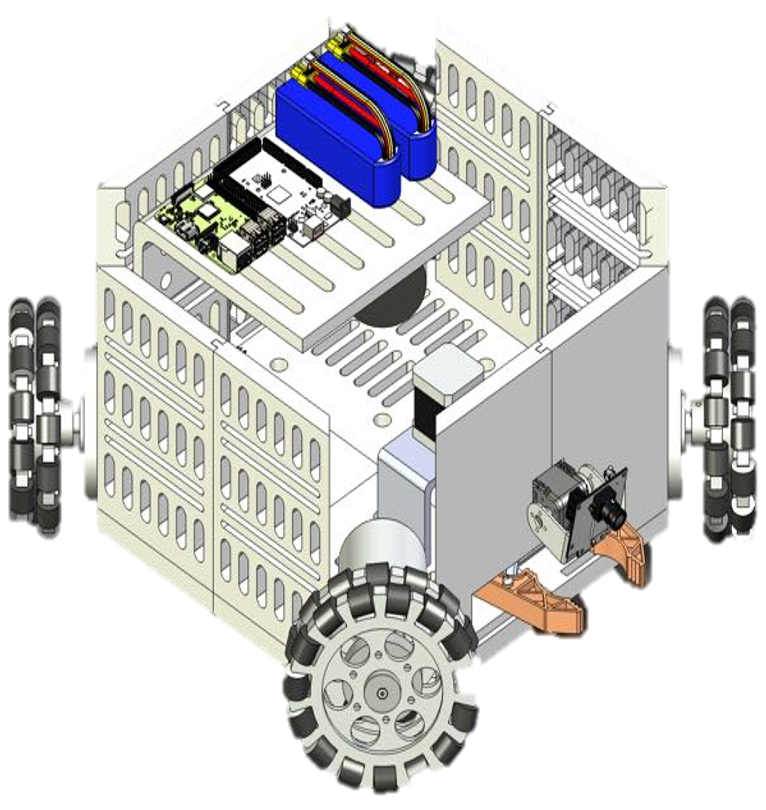
\includegraphics[scale = 0.8]{ourRobot3}
	%\caption{Integrated Development Environment (IDE)}
\end{figure}

\end{titlingpage}
\end{comment}

%\vspace{1.5cm}

\begin{titlingpage}

\newgeometry{top=2cm}

\begin {table}[H]
\centering
%\leftskip-3.8cm
\centering
\hspace{2cm}\hfil{\Huge\bf Plan de presupuesto para robot}
\leftskip-2cm\begin{tabular}{llllll}
    \toprule
    Descripción      &  No. de parte  & Proveedor & Cantidad & Precio unitario & Total (MXN)\\
    \midrule
    \fbox{\textsc{Material Electrónico}} \\
    \phantom{ZZ}Batería LiPo 5800 mAh 3S 30C    &   Z58003S-30  &   \href{https://hardtofind.com.mx/?htf=detalle&sku=Z58003S-30&busca=8&tl=Aeroplanos&tb=1&tg=HTF,AEROPLANO}{Hardtofind}  & 2 & \$1,345.99 & \$2,691.98 \\
    \phantom{ZZ}Cargador Balanceador LiPo 80W   &   9052000071-0  &  \href{https://hardtofind.com.mx/?htf=detalle&sku=9052000071-0&busca=26&tl=Simuladores&tb=2&tg=HTF,ACCESORIO,SIMULADOR} {Hardtofind}  & 1 & \$1,188.00 & \$1,188.00 \\
    \phantom{ZZ}Multiadaptador p/batería LiPo    &   015000151-0  &  \href{https://hardtofind.com.mx/?htf=detalle&sku=015000151-0&busca=1&tl=Aeroplanos&tb=1&tg=HTF,AEROPLANO} {Hardtofind}  & 1 & \$272.00 & \$272.00 \\
    \phantom{ZZ}Monitor de voltaje p/batería LiPo     &   67000001  &  \href{https://hardtofind.com.mx/?htf=detalle&sku=067000001&busca=26&tl=Simuladores&tb=2&tg=HTF,ACCESORIO,SIMULADOR} {Hardtofind}  & 1 & \$76.00 & \$76.00 \\
    \phantom{ZZ}\makecell{MOSFET 60V N-Channel QFET} & FQP30N06L &  \href{https://bit.ly/2wpkNXm} {Mouser}  & 20 & \$1.35 USD & \$515.82 \\
    \phantom{ZZ}\makecell{MOSFET 60V P-Channel QFET} & FQP47P06 &  \href{https://www.mouser.mx/ProductDetail/ON-Semiconductor-Fairchild/FQP47P06?qs=sGAEpiMZZMshyDBzk1\%2fWi1oKJWRB0GXwSn7Vcmu95\%2fU\%3d} {Mouser}  & 20 & \$2.47 USD & \$943.75 \\
    \phantom{ZZ}Transistor Output Optocouplers    &   CNY74-4H  &  \href{https://www.mouser.mx/ProductDetail/Vishay-Semiconductors/CNY74-4H?qs=sGAEpiMZZMteimceiIVCBwfsK9X9U0O6LWmHTDhgJbE\%3d} {Mouser}  & 15 & \$2.33 USD & \$667.70 \\
    \phantom{ZZ}Resistencias (diferentes valores)  &   N/A  &  \href{http://www.steren.com.mx/resistencia-de-carbon-de-1-2-watts-al-5-de-tolerancia.html} {Steren}  & 100 & \$1 & \$100 \\
    \phantom{ZZ}Base para circuito - 16 pines  &   COMCON00372  &  \href{http://www.techmake.com/00372.html} {TechMake}  & 10 & \$4 & \$40 \\
    \phantom{ZZ}Bloque terminal - 5mm, 2 pines  &   COMCON00514  &  \href{http://www.techmake.com/00514.html} {TechMake}  & 20 & \$5 & \$100 \\
    \phantom{ZZ}Arduino Uno R3 Generico &   AR-01  &  \href{https://troxino.com/producto/arduino-uno-r3-generico/1} {Troxino}  & 2 & \$150 & \$300 \\
    \phantom{ZZ}Protoboard 830 puntos &   PB-001  &  \href{https://troxino.com/producto/protoboard-830-puntos/24} {Troxino}  & 2 & \$50 & \$100 \\
    \phantom{ZZ}Modulo Pololu A4988 &   POL4988  &  \href{https://troxino.com/producto/modulo-pololu-a4988/109} {Troxino}  & 3 & \$35 & \$105 \\
    \phantom{ZZ}Placa Fenolica de Cobre &   575493101  & \href{https://articulo.mercadolibre.com.mx/MLM-575493101-placa-fenolica-de-cobre-doble-cara-10x15-2-pzas-_JM} {Mercado Libre}  & 2 & \$49 & \$98 \\
    \phantom{ZZ}Raspberry Pi 3 B+ &   RB-018  & \href{https://troxino.com/producto/raspberry-pi-3-b-2018/251} {Troxino}  & 1 & \$1,390 & \$1,390 \\
    \phantom{ZZ}Disipador TO-22 &   TO-220 C/C  & \href{http://www.steren.com.mx/disipador-electronico-para-to-22.html} {Steren}  & 35 & \$26 & \$910 \\
    
    \phantom{ZZ}Cable Calibre 16 AWG 100mts &   N/A  & \href{https://articulo.mercadolibre.com.mx/MLM-575742203-rollo-100-mts-cable-thw-calibre-16-kobrex-varios-colores-_JM} {MercadoLibre}  & 1 & \$584 & \$584 \\
    \phantom{ZZ}Alambre Calibre 22 AWG 100mts &   N/A & \href{https://articulo.mercadolibre.com.mx/MLM-550889888-cable-protoboard-100-mts-alambre-estanado-calibre-22-awg-_JM} {MercadoLibre}  & 1 & \$300 & \$300 \\
    \textsc{Subtotal} & & & & & \fbox{\$10,382.25}\\
    \midrule
    \fbox{\textsc{Sensores}} \\
    \phantom{ZZ} Camara Pixy CMUcam5 Sensor  &   SENLIM00564  &  \href{http://www.techmake.com/00564.html} {Techmake}  & 1 & \$2,500 & \$2,500\\
    \phantom{ZZ} Acelerómetro Analógico de 3 Ejes &   SE-009  &  \href{https://troxino.com/producto/acelerometro-analogico-de-3-ejes-mma7361/34} {Troxino}  & 1 & \$95 & \$95\\
    \phantom{ZZ} Giroscopio Analogico 3 ejes & GY-521 & \href{http://semty.mx/index.php?id_product=2168&controller=product} {Semty}  & 1 & \$80 & \$80\\
    \phantom{ZZ} Camara para Raspberry Pi v1.3  & RB-003 & \href{https://troxino.com/producto/camara-para-raspberry-pi-v1-3-5mp-1080p/57} {Troxino}  & 1 & \$290 & \$290\\
    \textsc{Subtotal} & & & & & \fbox{\$2,965.00}\\
    \midrule
    \fbox{\textsc{Actuadores}} \\
    \phantom{ZZ}Kit de Pinza Estandar &  ROBOTH00398  &  \href{http://www.techmake.com/productos/robotica/robotica-otros/00398.html} {Techmake}  & 2 & \$340 & \$680\\
    \phantom{ZZ}Servo Hitec HS-422 Estandar &  ROBMOT00125  &  \href{http://www.techmake.com/00125.html} {Techmake}  & 2 & \$350 & \$700\\
    \phantom{ZZ}Motor DC Alto Par Torque &  SKU: 180  &  \href{https://www.lionchipmexico.com/product-page/motor-dc-alto-par-torque-43-kg-12v-47-rpm-robot-32-mm} {Lionchip}  & 4 & \$514 & \$2,056\\
    \phantom{ZZ}Motor a pasos NEMA 17 &   SM-08  &  \href{https://troxino.com/producto/motor-a-pasos-nema-17-17hs4401-4kg-cm/123} {Troxino}  & 1 & \$270 & \$270\\
    \phantom{ZZ}100mm Omnidirectional Wheel &  RB-Nex-08  &  \href{https://www.robotshop.com/en/100mm-omnidirectional-wheel-brass-bearing-rollers.html} {Roboshop}  & 4 & \$20.16 USD & \$1,540.57\\
    \textsc{Subtotal} & & & & & \fbox{\$5,246.57}\\
    \midrule
    \fbox{\textsc{Herramientas}} \\
    \phantom{ZZ} Cautín &   CAU-130   &  \href{http://www.steren.com.mx/cautin-tipo-lapiz-de-40-watts.html} {Steren}  & 2 & \$199 & \$398\\
    \phantom{ZZ} Desoldador de Succión &   CAU-170   &  \href{http://www.steren.com.mx/desoldador-chico-de-succion-de-aire.html} {Steren}  &1 & \$69 & \$69\\
    \phantom{ZZ} Soldadura &   SOL60-100   &  \href{http://www.steren.com.mx/rollo-de-100-gramos-de-soldadura-con-aleacion-estano-plomo-60-40.html} {Steren}  &1 & \$140 & \$140\\
    \phantom{ZZ} Pinza de Punta &   TOLHTO00188   &  \href{http://www.techmake.com/00188.html} {Techmake}  &1 & \$55 & \$55\\
    \phantom{ZZ} Pinza de Corte &   TOLHTO00187   &  \href{http://www.techmake.com/00187.html} {Techmake}  &1 & \$55 & \$55\\
    \phantom{ZZ} Desarmadores Kit &   HER-192   &  \href{http://www.steren.com.mx/juego-de-desarmadores-de-precision-31-en-1.html} {Steren}  &1 & \$195& \$195\\
    \phantom{ZZ} Juego Dados &   101555224   &  \href{https://www.lowes.com.mx/llaves-y-dados/4664-juego-de-dados-truper-39-piezas.html} {Lowes’}  &1 & \$29& \$295\\
    \phantom{ZZ} Pack tornillos y tuercas M3 10 mm &   N/A   &  \href{https://www.taloselectronics.com/products/paquete-con-10-tornillos-m3-10-mm-y-10-tuercas-m3} {Taloselectronics}  &4 & \$35& \$140\\
    \phantom{ZZ} Pack tornillos y tuercas M3 30 mm &   N/A &  \href{https://www.taloselectronics.com/products/paquete-con-10-tornillos-m3-30-mm-y-10-tuercas-m3} {Taloselectronics}  &4 & \$25& \$100\\
    %Materials awaiting delivery             &              & 20,779,350.27           &  22,074,223.60 \\
    %Materials still to be ordered by HS     &                                                         \\
    %\phantom{ZZ}Mechanical                  &    158,030.10&                         &      38,351.40 \\
    %\phantom{ZZ}Electrical                  &    344,162.53&                         &     287,394.98 \\
    %LPOs to be released by HLG              &  3,337,934.08&                         &   1,276,883.12 \\ 
    %Materials with HOK issues etc.,         & 22,692,102.00&                         &  22,692,102.00 \\                                   \\   
    %\textsc{Total Projected Materials Cost} &              &197,660,733.55           & 197,660,733.55 \\

    %Materials used in Phase II              &(2,000,000.00)&\\
    %Materials damaged in fire               &(2,130,000.00)&\\
    %Scrap recovery                          &(2,000,000.00)&\\
    %Salvage value on ending stock           &(3,000,000.00)&\\
    %\textsc{Sub-total}                      &(9,130,000.00)&\\
    \textsc{Subtotal} & & & & & \fbox{\$1,447.00}\\
    \midrule

    \textsc{Costo total del proyecto} & & & & & \fbox{\$20,040.82}\\
    \bottomrule                
    \end{tabular}
\end{table}
\end{titlingpage}

\end{document}
